\documentclass{article}

\usepackage[dutch]{babel}
\usepackage{epsfig}
\usepackage{verbatim}
\usepackage{moreverb}
\usepackage{float}
\usepackage{graphicx}
\usepackage{framed}
\usepackage{chngcntr}
\usepackage{enumitem}
\usepackage{verbdef}
\usepackage{mathtools}
\usepackage{amsmath}
\usepackage[font=bf]{caption}

\author{Peter van Dijk \& Elizabeth Schermerhorn}
\date{\today}
\title{Localisatie met Arduino's op basis van vier bakens}
\begin{document}
\maketitle
\newpage
\tableofcontents
\clearpage
\section{Inleiding}
In deze paper zal een localisatie algoritme besproken worden. De localisatie zal gedaan worden op basis van vier bakens die een ultrasoon geluid uitzenden en een arduino met een ultrasoon ontvanger. Het doel van dit experiment is om binnen een 5m bij 5m veld de positie zo nauwkeurig mogelijk proberen te bepalen. Aan de hand van het ultrasone geluid in combinatie met een GPS-bepalings algoritme wordt nauwkeurig bepaald wat de co\"{o}rdinaten zijn. 


\section{Probleemstelling}
De onderzoeksvraag die hier centraal staat: \textit{"Een algoritme opstellen waarmee met trilateratie de positie bepaald kan worden met 5 \% nauwkeurigheid."}
De hypothese is dat dit een uitdaging is, er zijn veel factoren die van invloed zijn op de berekening van de trilateratie. Twee belangrijke factoren zullen de geluidssnelheid worden en de overflow(Getallen zijn te groot om te representeren) in arduino zijn. 

\section{Gerelateerd werk}
Op dit gebied is er al veel onderzoek verricht. Hierdoor is er veel werk wat gebruikt kan worden bij het onderzoek. Aangezien dit een onderzoek is wat al vele malen is uitgevoerd is er veel gerelateerd werk wat is gebruikt in dit onderzoek. In deze twee papers worden er globale localisatie systemen beschreven en hoe deze gebruik maken van externe factoren. In de volgende twee papers worden er GPS-bepalings algoritmen gepresenteerd waarmee de exacte locatie bepaald kan worden. In de eerste twee papers worden twee manieren toegelicht waarop localisering mogelijk is. In [http://www.cl.cam.ac.uk/research/dtg/www/publications/public/files/tr.97.10.pdf] worden twee manieren beschreven, namelijk:
\begin{itemize}
	\item Active badges
	\item ParcTab
\end{itemize}

Active badges is gebasseerd op het periodiek verzenden van informatie naar iedereen. Door -bijvoorbeeld een gebouw - heen zijn er overal sensoren geplaatst die luisteren naar berichten die worden verstuurd door badges. Door vast te stellen welke sensoren het signaal van welke badge hebben ontvangen is het mogelijk een grove schatting te g
even van de locatie van de badge.
\newline 

ParcTab is een PDA die gebruik maakt van infrarood voor het netwerk.Wat betreft de localisatie bepaling lijkt deze heel veel op de badges die hierboven staan beschreven. Er worden berichten verstuurd en afhankelijk van welke sensor deze ontvangen wordt de locatie bepaald. Een groot verschil is dat de ParcTab is bedoeld voor veel meer en intensiever gebruik dan alleen de localatie berekenen. 

In de laatste twee papers, [http://en.wikipedia.org/wiki/Trilateration] en [Localization and positioning, CH. 9] worden er twee manieren besproken waarop de GPS positie bepaald kan worden. 

In hoofdstuk 9 van Localization and positioning wordt er ook gebruik gemaakt van bakens die een signaal uitzenden. Er moet eerst berekend worden wat de afstand is tot de verschillende bakens. Voor dit algoritme is het van belang dat er minimaal tot drie bakens de locatie bekend is. Wanneer de afstand tot drie bakens bekend is wordt er gebruik gemaakt van matrixberekeningen om de locatie te bepalen. Dit is de implementatie die ook is gebruikt in het experiment wat in deze paper is gemaakt.
\newline
Een tweede GPS-positie bepaling die gebruikt zou kunnen worden heet triangulation. Ook hier wordt gebruik gemaakt van de afstand tot de bakens die een signaal verzenden. Dit algoritme lijkt veel op het algoritme uit CH9 maar hier wordt gebruik gemaakt van de berekening van cirkels waardoor er geen matrixberekeningen nodig zijn. 




\section{Instellingen}
Om deze hypothesen te toetsen moeten er metingen gedaan worden. Hier zijn verschillende zaken van belang. 
\begin{itemize}
	\item De gebruikte hardware
	\item De gebruikte software
	\item De instellingen/vastgestelde constanten
	\item De onderzoeksopstelling
\end{itemize}

%De gebruikte hardware
\subsection{De hardware}
\subsubsection{Ontvanger}
De Hardware die gebruikt is bij het ontvangen van de signalen is een Arduino UNO en een Nordic nRF24L01 draadloze transceiver in combinatie met een ultrasoonontvanger. In Fig. \ref{voorkant} en \ref{achterkant} staat de gebruikte arduino vanuit twee posities bekeken.\\ 
\begin{figure}[h]
\centering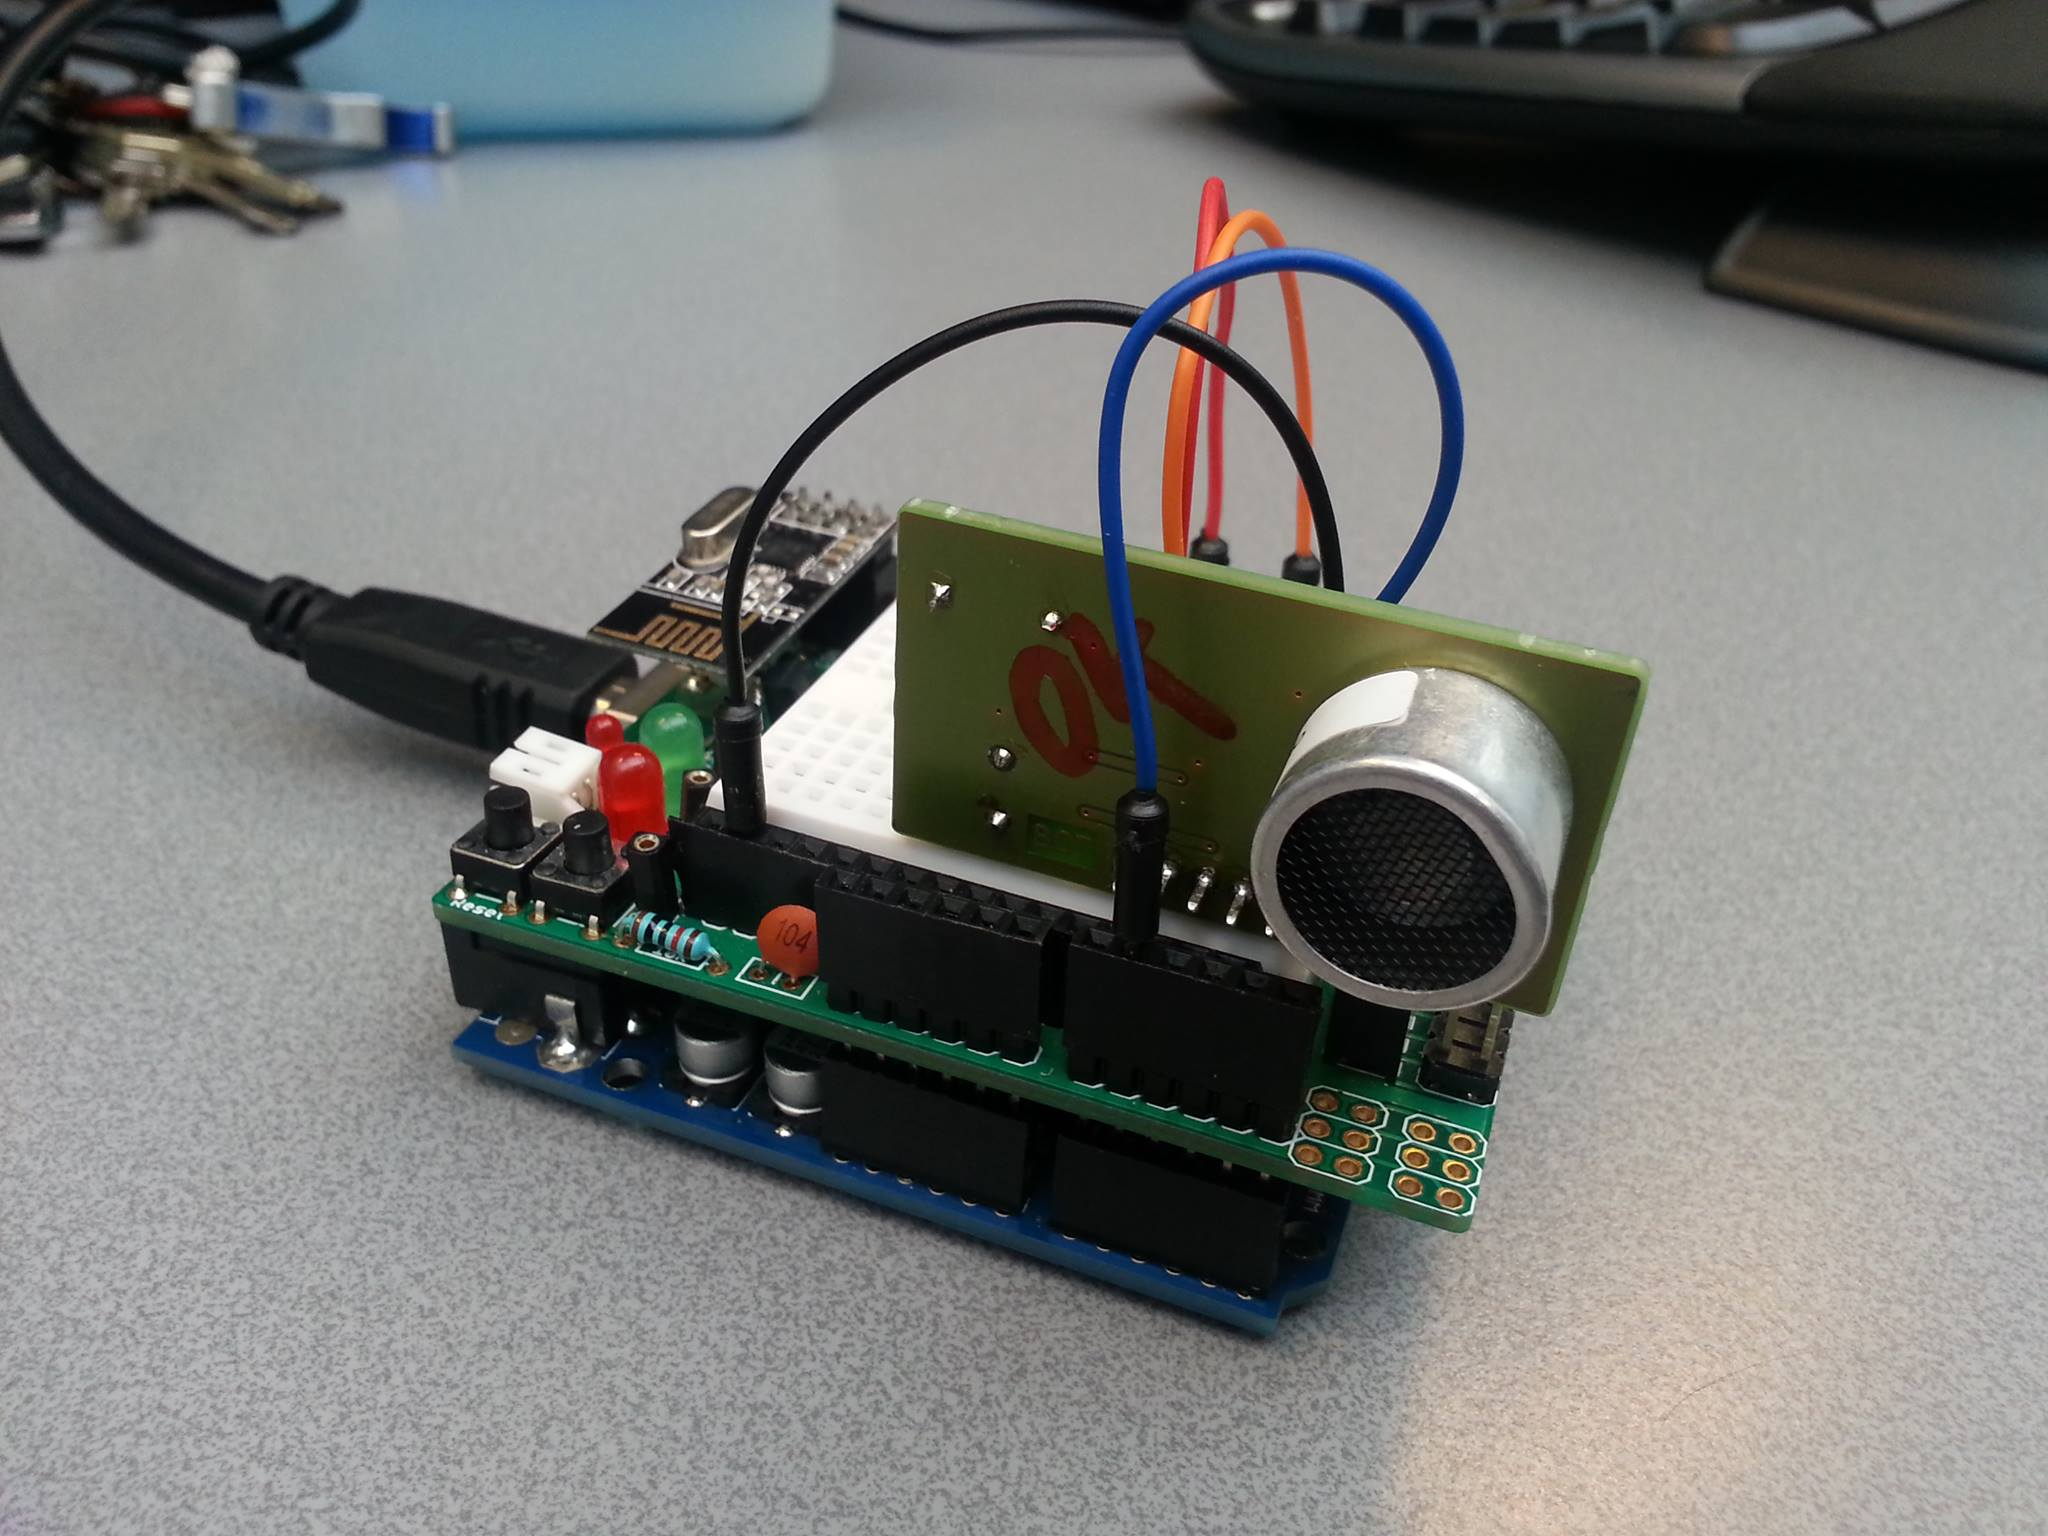
\includegraphics[scale=0.06]{voorkant.jpg}
\caption{De gebruikte arduino(voorkant)}
\label{voorkant}
\end{figure}
\begin{figure}[h]
\centering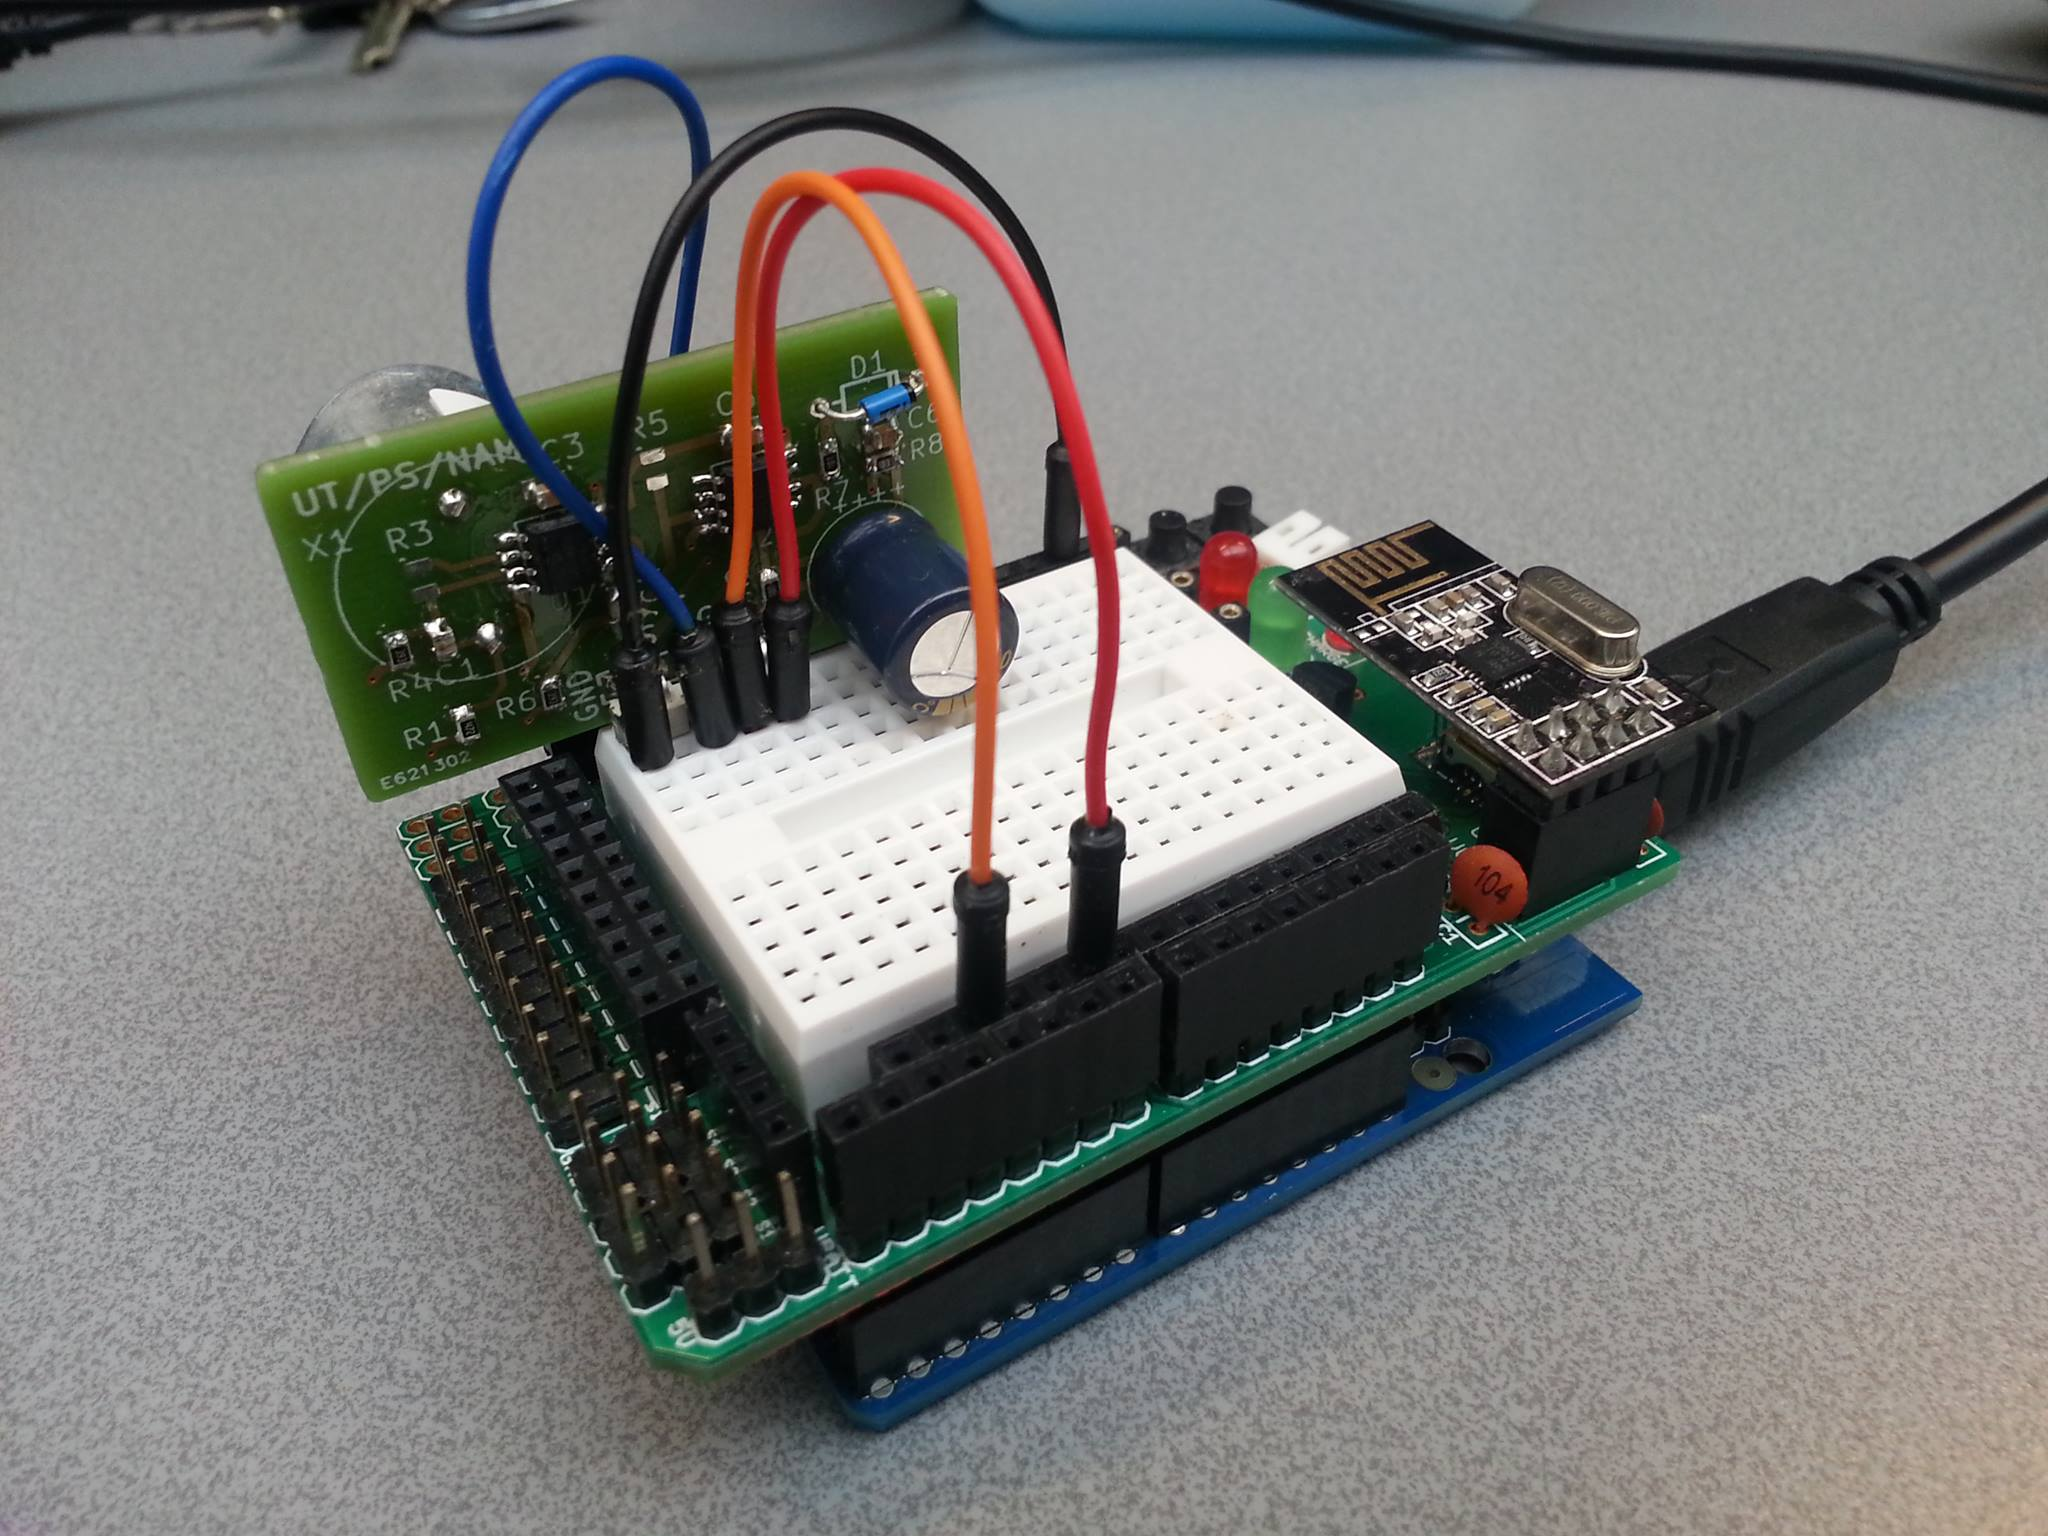
\includegraphics[scale=0.06]{achterkant.jpg}
\caption{De gebruikte arduino(achterkant)}
\label{achterkant}
\end{figure}

\subsubsection{zender}
Als zender is er gebruik gemaakt van vier bakens die een ultrasoon geluid uitzenden. Het signaal van deze bakens wordt verstuurd in de richting waarin ze wijzen. In Fig. \ref{baken} staat een schematische weergave van hoe een baken eruitziet. Er is duidelijk te zien dat het ultrasone geluid \'{e}\'{e}n kant uitgezonden wordt.
\begin{figure}[h]
\centering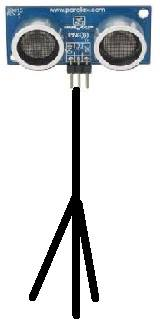
\includegraphics[scale=0.5]{Ultrasonic-Range-Finderv2.jpg}
\caption{schematische baken}
\label{baken}
\end{figure}
%de gebruikte software
\subsection{De software}
Om de hardware te gebruiken wordt gebruik gemaakt van de opensourcesoftwarebibliotheek voor de Arduino, die te vinden is op: \begin{verbatim}http://maniacbug.github.io/RF24/ \end{verbatim} 
Met deze software kunnen de radio en ontvanger aangestuurd worden en kunnen pakketjes worden verzonden en ontvangen. De radio luistert en verstuurt pakketten over een bepaald kanaal. Het is van belang dat de radio's hetzelfde kanaal gebruiken, zodat ze met elkaar kunnen communiceren. De kanalen hebben een nummer van 0 tot en met 125. De radio heeft de volgende instellingen nodig:
\begin{itemize}
	\item Kanaal 76 
	\item Automatisch herverzenden Uit
	\item Transmissiesnelheid: 2 Mbps
	\item Adres verzendende pipe: 0xdeadbeefa1LL
	\item Payload-grootte 1 byte
\end{itemize}
De ultrasoon ontvanger moet op een bepaalde manier aangesloten worden zodat deze geluid kan ontvangen:
\newline
\begin{tabular}{l| l}
\hline
afkorting & Wijze van aansluiten \\ \hline
E & Verbinden met GND van Arduino \\
GN & Verbinden met 5V van Arduino \\
++ & Verbinden met 5V van Arduino \\
GND & Verbinden met Ground van Arduino \\
S & niet aansluiten \\
\end{tabular}
\\
\\
Om de tests te kunnen uitvoeren is er gebruik gemaakt van vier bakens die met een bepaald patroon informatie verzenden. In fig.  \ref{uitzenden_bakens} is schematisch weergegeven hoe de signaal verzending werkt. In het schema zijn vier dezelfde iteraties te zien. Omdat er gebruik wordt gemaakt van vier bakens staan er vier berichten in het schema weergegeven. 
\begin{figure}[h]
\centering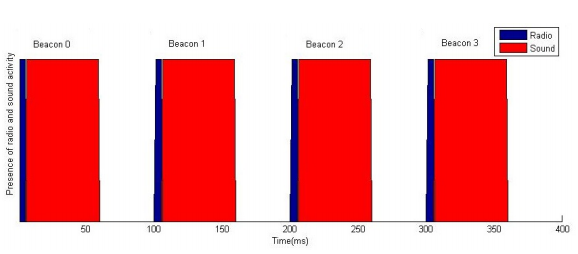
\includegraphics[]{berichten_bakens.png}
\caption{Het signaal van de bakens}
\label{uitzenden_bakens}
\end{figure}


\section{Het algoritme}
Het algoritme wat ge\"{i}mplementeerd is, bestaat uit twee verschillende onderdelen. Het bestaat uit een deel afstand berekenen tot de verschillende bakens, en de uiteindelijke GPS-bepaling. 
Deze twee onderdelen zullen apart besproken worden voor de overzichtelijkheid.
	
\subsection{Afstand bepalen tot aan de bakens}
	Zoals te zien is in Fig.\ref{uitzenden_bakens} wordt er eerst een radio signaal verstuurd gevolgd door een ultrasoon signaal. Het versturen van een ultrasoon bericht wordt door een master-baken bepaald. Als eerste wordt er door de master-baken een radio bericht uitgezonden naar iedereen met het bericht welke baken mag sturen. Omdat dit een radiosignaal is gaat dit met de snelheid van het licht, hierdoor is het verschil tussen de verschillende nodes die het op verschillende momenten ontvangen verwaarloosbaar. Op het moment dat het radio signaal ontvangen wordt, begint de desbetreffende baken direct met een ultrasoon geluid versturen. Doordat bekent is dat dit meteen gebeurt wordt er bijgehouden hoelang het duurt tussen het ontvangen van het radiosignaal en het ontvangen van ultrasoon geluid. Op het moment dat het bericht wordt ontvangen wordt er met behulp van de geluidssnelheid berekend wat de afstand tot het baken is. Met de formule:\newline
	$ d_b = (T_u- T_r) * g $
	\newline\newline
	$ d_b$ = afstand tot baken\newline
	$T_u$ = Tijd ontvangen ultrasoon geluid\newline
	$T_r$ = Tijd ontvangen radio\newline
	$g$ = geluidssnelheid\newline
	
	Het is van belang om een juiste geluidssnelheid te kiezen bij de omgeving waarin het systeem staat, de afwijkingen kunnen groot zijn. Dit proces van luisteren en berekenen herhaalt zich oneindig lang zodat wanneer de node in beweging is er nog steeds een correcte locatie berekend kan worden. 
	
\subsection{Trilateration}
Nu van alle vier de bakens bekend is wat hun afstand is tot de node kan door middel van matrixberekeningen de positie worden bepaald. Hierbij is er gebruik gemaakt van [iets]. 
De volgende berekening is gebruikt bij het berekenen van de locatie: \newline
$2*\begin{bmatrix}
       x_3 - x_1 & y_3 - y_1 \\
       x_3 - x_2 & y_3 - y_2 \\          
                
     \end{bmatrix}
     \begin{bmatrix}
       x_u \\          
       y_u \\         
     \end{bmatrix}
=\begin{bmatrix}
       (r_1^2 - r_3^2) - (x_1^2 - x_3^2) - (y_1^2 - y_3^2) \\
       (r_2^2 - r_3^2) - (x_2^2 - x_3^2) - (y_2^2 - y_3^2) \\
     \end{bmatrix}$     
\newline
\newline
De argumenten in bovenstaande berekening betekenen: \newline
$x_u$ = de te berekenen x-co\"{o}rdinaat van de arduino.\newline
$y_u$ = de te berekenen y-co\"{o}rdinaat van de arduino.\newline
$x_x$ = het x-co\"{o}rdinaat van baken x.\newline
$y_x$ = het y-co\"{o}rdinaat van baken x.\newline
$r_x$ = de afstand van de arduino tot aan baken x.\newline
\newline
Doordat de te berekenen x en y co\"{o}rdinaten aan de linkerkant genest in de formule staan was het nodig om deze om te schrijven. De volgende hulpberekeningen volgden daaruit: \newline
$c_1 = (((r_1*r_1)-(r_3*r_3))-((x_1*x_1)-(x_3*x_3))-((y_1*y_1)-(y_3*y_3)))/2 $
\newline
\newline
$c_2 = (((r_2*r_2)-(r_3*r_3))-((x_2*x_2)-(x_3*x_3))-((y_2*y_2)-(y_3*y_3)))/2 $
\newline
\newline
$n =(-((y_3-y_1)*10000)/(x_3-x_1)) $
\newline
\newline
$m = ((c_1*10000)/(x_3-x_1)) $
\newline
\newline
$y = ((c_2*10000) - m*(x_3-x_2))/(n*(x_3-x_2) + (10000*(y_3-y_2))) $
\newline
\newline
$x = ((n*y)+m)/10000 $
\newline
\newline
Er wordt eerst vermenigvuldigd met 10000 om later weer te delen door 10000. Dit is gedaan omdat arduino's niet goed rekenen met floats, de oplossing hiervoor was de getallen groot houden zodat er geen komma getallen ontstaan. 
Door de formules in deze volgorde uit te voeren worden de x en y uiteindelijk berekend. Doordat de afstand tot aan de bakens elke 400ms opnieuw wordt berekend geldt dit ook voor de x en y co\"{o}rdinaten. Elke keer als er een nieuwe afstand bekend is worden bovenstaande formules opnieuw berekend. 

\section{Testopstelling en metingen}
Om de implementatie te testen is er gebruik gemaakt van een testopstelling zoals die in Fig. \ref{Meetopstelling} staat weergegeven.
\begin{figure}[h] 
\centering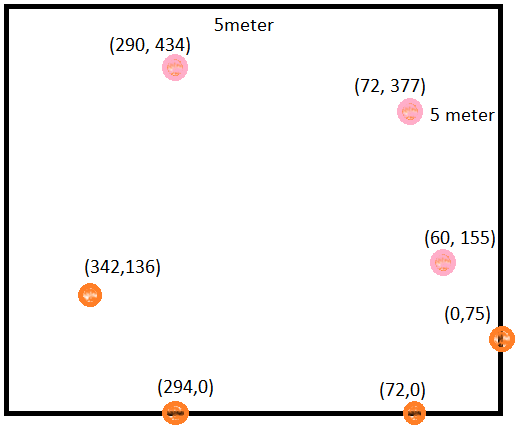
\includegraphics[scale=0.5]{Meetopstelling.png}
\caption{Meetopstelling}
\label{Meetopstelling}
\end{figure}
De unisoonontvangers waarmee de signalen van de bakens worden ontvangen werden na vijf meter zeer onnauwkeurig dus is ervoor gekozen om binnen een veld van 5 bij 5 meter te werken. In het schema staan de vier bakens aangegeven met de oranje stippen samen met hun co\"{o}rdinaten. Met de roze stippen worden de testlocaties bedoeld waarop is getest. De bakens die zijn gebruikt versturen alleen signalen in de richting waarin ze wijzen. Hierdoor is het niet mogelijk correcte gegevens te verkrijgen wanneer er vanachter de bakens wordt gemeten. 
\newline
Tijdens het testen wordt een arduino met radio en unisoon ontvanger op een bepaald co\"{o}rdinaat geplaatst. Het is belangrijk dat deze locatie precies is anders ontstaat er een afwijking tussen de meetresultaten en de verwachte waarde. 
Het is van belang bij het testen dat er gebruik wordt gemaakt van een "schoon" grid. Dit houdt in, geen obstakels die de metingen zouden kunnen verstoren zoals mensen die erdoorheen lopen. Alle tests zijn "schoon" uitgevoerd. 
Op de volgende locaties zijn de volgende tests uitgevoerd.
\newline
Test1: De arduino wordt op het co\"{o}rdinaat (290, 434) geplaatst. \newline
Test2: De arduino wordt op het co\"{o}rdinaat (60, 155) geplaatst. \newline
Test3: De arduino wordt op het co\"{o}rdinaat (72, 377) geplaatst. \newline
Verwacht wordt dat de metingen zeer nauwkeurig zullen zijn < 5\% afwijking. 
In Appendix Meetresultaten staan alle meetresultaten van de drie tests verwerkt. In de tabellen staat de laatste waarde voor het gemiddelde wat werd berekend door de arduino. de overige waarden zijn 25 gemeten waarden op die positie. Te zien is dat de metingen niet hetzelfde zijn, ze fluctueren binnen een interval. Een paar redenen hiervoor zijn: 
\begin{itemize}
	\item De node zit niet vast, iemand houdt de node vast en hier kan een paar centimeter verschil in zitten.
	\item De geluidssnelheid is erg belangrijk voor de berekening en het is mogelijk dat voor die omgeving op dat moment de verkeerde geluidssnelheid was ingevoerd. 
	\item De ultrasoon ontvanger ontvangt ook echo's die weerkaatsen op objecten. Deze foutieve metingen worden meegenomen in de berekening waardoor de waarde niet meer klopt. 
	\item Hoewel er op gelet is dat er niemand door het grid heen loopt tijdens de metingen is het moeilijk om alles tegelijk in de gaten te houden en zou het kunnen voorkomen dat iemand erdoorheen gelopen is.
\end{itemize}

\section{Conclusie}
De onderzoeksvraag die hier centraal staat: \textit{"Een algoritme opstellen waarmee met trilateratie de positie bepaald kan worden met 5 \% nauwkeurigheid."} Dit experiment is een succes, het is gelukt om een algoritme te ontwikkelen en implementeren waarmee de marge <=5\% is. Hiermee is het experiment een succes.
\subsection{Aanbevelingen} 
 Voor een vervolgonderzoek zou er naar de volgend punten gekeken kunnen worden.
 \begin{itemize}
 	\item de overflow die ontstaat met het rekenen met integers, op het moment dat de arduino verder staat dan 6 meter bij de bakens vandaan ontstaat er overflow.
 	\item betere bakens en ontvangers, de signalen worden minder na 6 meter
 	\item een algoritme ontwerpen wat beter tegen verstoringen in het veld kan. 
 \end{itemize}
\clearpage
\appendix
\counterwithin{figure}{section}
\section{Code Trilateration}
\verbatiminput{./location/location.ino}
\newpage
\section{Meetresultaten}
\begin{tabular}{ |l|l| }
  \hline
  \multicolumn{2}{|c|}{(290, 434)} \\
  \hline
  x-coordinaat & y-coordinaat \\ \hline
     294 & 434\\ \hline
     296 & 445\\ \hline
     296 & 441\\ \hline
     293 & 434\\ \hline
     295 & 436\\ \hline
     293 & 434\\ \hline
     297 & 439\\ \hline
     294 & 432\\ \hline
     293 & 449\\ \hline
     292 & 449\\ \hline
     292 & 449\\ \hline
     293 & 449\\ \hline
     292 & 439\\ \hline
     294 & 439\\ \hline
     286 & 433\\ \hline
     286 & 433\\ \hline
     292 & 436\\ \hline
     291 & 435\\ \hline
     289 & 429\\ \hline
     295 & 436\\ \hline
     293 & 444\\ \hline
     293 & 435\\ \hline
     294 & 451\\ \hline
     293 & 433\\ \hline
     293 & 433\\ \hline
     288 & 440\\ \hline\hline
     292,9 & 439,1 \\ \hline
\end{tabular}
\begin{tabular}{ |l|l| }
  \hline
  \multicolumn{2}{|c|}{(60, 155)} \\
  \hline
  x-coordinaat & y-coordinaat \\ \hline
     59 & 137\\ \hline
     57 & 147\\ \hline
     58 & 154\\ \hline
     58 & 151\\ \hline
     60 & 157\\ \hline
     60 & 148\\ \hline
     60 & 154\\ \hline
     62 & 147\\ \hline
     63 & 151\\ \hline
     62 & 147\\ \hline
     61 & 137\\ \hline
     60 & 154\\ \hline
     60 & 150\\ \hline
     60 & 152\\ \hline
     59 & 152\\ \hline
     60 & 154\\ \hline
     61 & 151\\ \hline
     60 & 152\\ \hline
     62 & 155\\ \hline
     61 & 152\\ \hline
     61 & 155\\ \hline
     61 & 149\\ \hline
     61 & 155\\ \hline
     61 & 154\\ \hline
     60 & 152\\ \hline
     63 & 156\\ \hline\hline
     60,4  & 151,8 \\ \hline
\end{tabular}
\begin{tabular}{ |l|l| }
  \hline
  \multicolumn{2}{|c|}{(72, 377)} \\
  \hline
  x-coordinaat & y-coordinaat \\ \hline
     75 & 378\\ \hline
     77 & 383\\ \hline
     76 & 382\\ \hline
     76 & 381\\ \hline
     75 & 378\\ \hline
     74 & 374\\ \hline
     74 & 377\\ \hline
     75 & 378\\ \hline
     76 & 382\\ \hline
     77 & 387\\ \hline
     76 & 388\\ \hline
     78 & 382\\ \hline
     74 & 387\\ \hline
     76 & 378\\ \hline
     74 & 382\\ \hline
     76 & 381\\ \hline
     77 & 377\\ \hline
     75 & 382\\ \hline
     77 & 377\\ \hline
     75 & 380\\ \hline
     76 & 374\\ \hline
     73 & 382\\ \hline
     75 & 377\\ \hline
     74 & 376\\ \hline
     77 & 378\\ \hline
     78 & 380\\ \hline\hline
     75,6 & 379,5 \\ \hline 
\end{tabular}
\newline
\begin{tabular}{ |l|p{3,33cm}| }
  \hline
  \multicolumn{2}{|c|}{\%- afwijking(290, 434)} \\
  \hline
  x & 0,34 \\ \hline
  y & 0,011 \\ \hline
\end{tabular}
\begin{tabular}{ |l|p{3,33cm}| }
  \hline
  \multicolumn{2}{|c|}{\%- afwijking (60, 155)} \\
  \hline
  x & 0,006 \\ \hline
  y & 2,581 \\ \hline
\end{tabular}
\begin{tabular}{ |l|p{3,33cm}| }
  \hline
  \multicolumn{2}{|c|}{\%- afwijking(72,377)} \\
  \hline
  x & 5 \\ \hline
  y & 0,531 \\ \hline
\end{tabular}

\end{document}